\documentclass[final]{article}

\PassOptionsToPackage{numbers,compress}{natbib}
\usepackage{APS360}
\usepackage{amsmath}
\usepackage[utf8]{inputenc}
\usepackage[T1]{fontenc}
\usepackage{hyperref}
\usepackage{url}
\usepackage{booktabs}
\usepackage{amsfonts}
\usepackage{nicefrac}
\usepackage{microtype}
\usepackage{xcolor}
\usepackage{graphicx}
\usepackage{caption}
\usepackage{wrapfig}
\captionsetup{font=small,labelfont=bf}
\DeclareMathOperator{\sinc}{sinc}

% TODO markers -- remove once resolved.
\newcommand{\todo}[1]{\textcolor{red}{\textbf{[TODO: #1]}}}

\begin{document}
\vspace{-26pt}

\href{https://github.com/noshou/APS360/tree/main}{\textbf{Github Repo}}\hfill
\href{https://noshou.github.io/APS360/}{\textbf{Live Demo}}

%==============================================================================
\section{Introduction}
%==============================================================================
X-ray/small-angle scattering intensity $I(q)$ is a highly non-linear,  1-D fingerprint of a molecule's 3-D
shape, used throughout structural biology, materials science, and chemistry to characterize
large, disordered, and dynamic molecules. The exact calculation, the Debye equation, sums 
every pairwise interatomic interaction at $O(N^2)$ cost, which is prohibitive for 
large structures. This project asks whether a GNN can learn $I(q)$ directly from atomic coordinates 
and element identities via a learned $O(N)$ model.

%==============================================================================
\section{Illustration / Figure}
%==============================================================================
\begin{figure}[h]
    \centering
    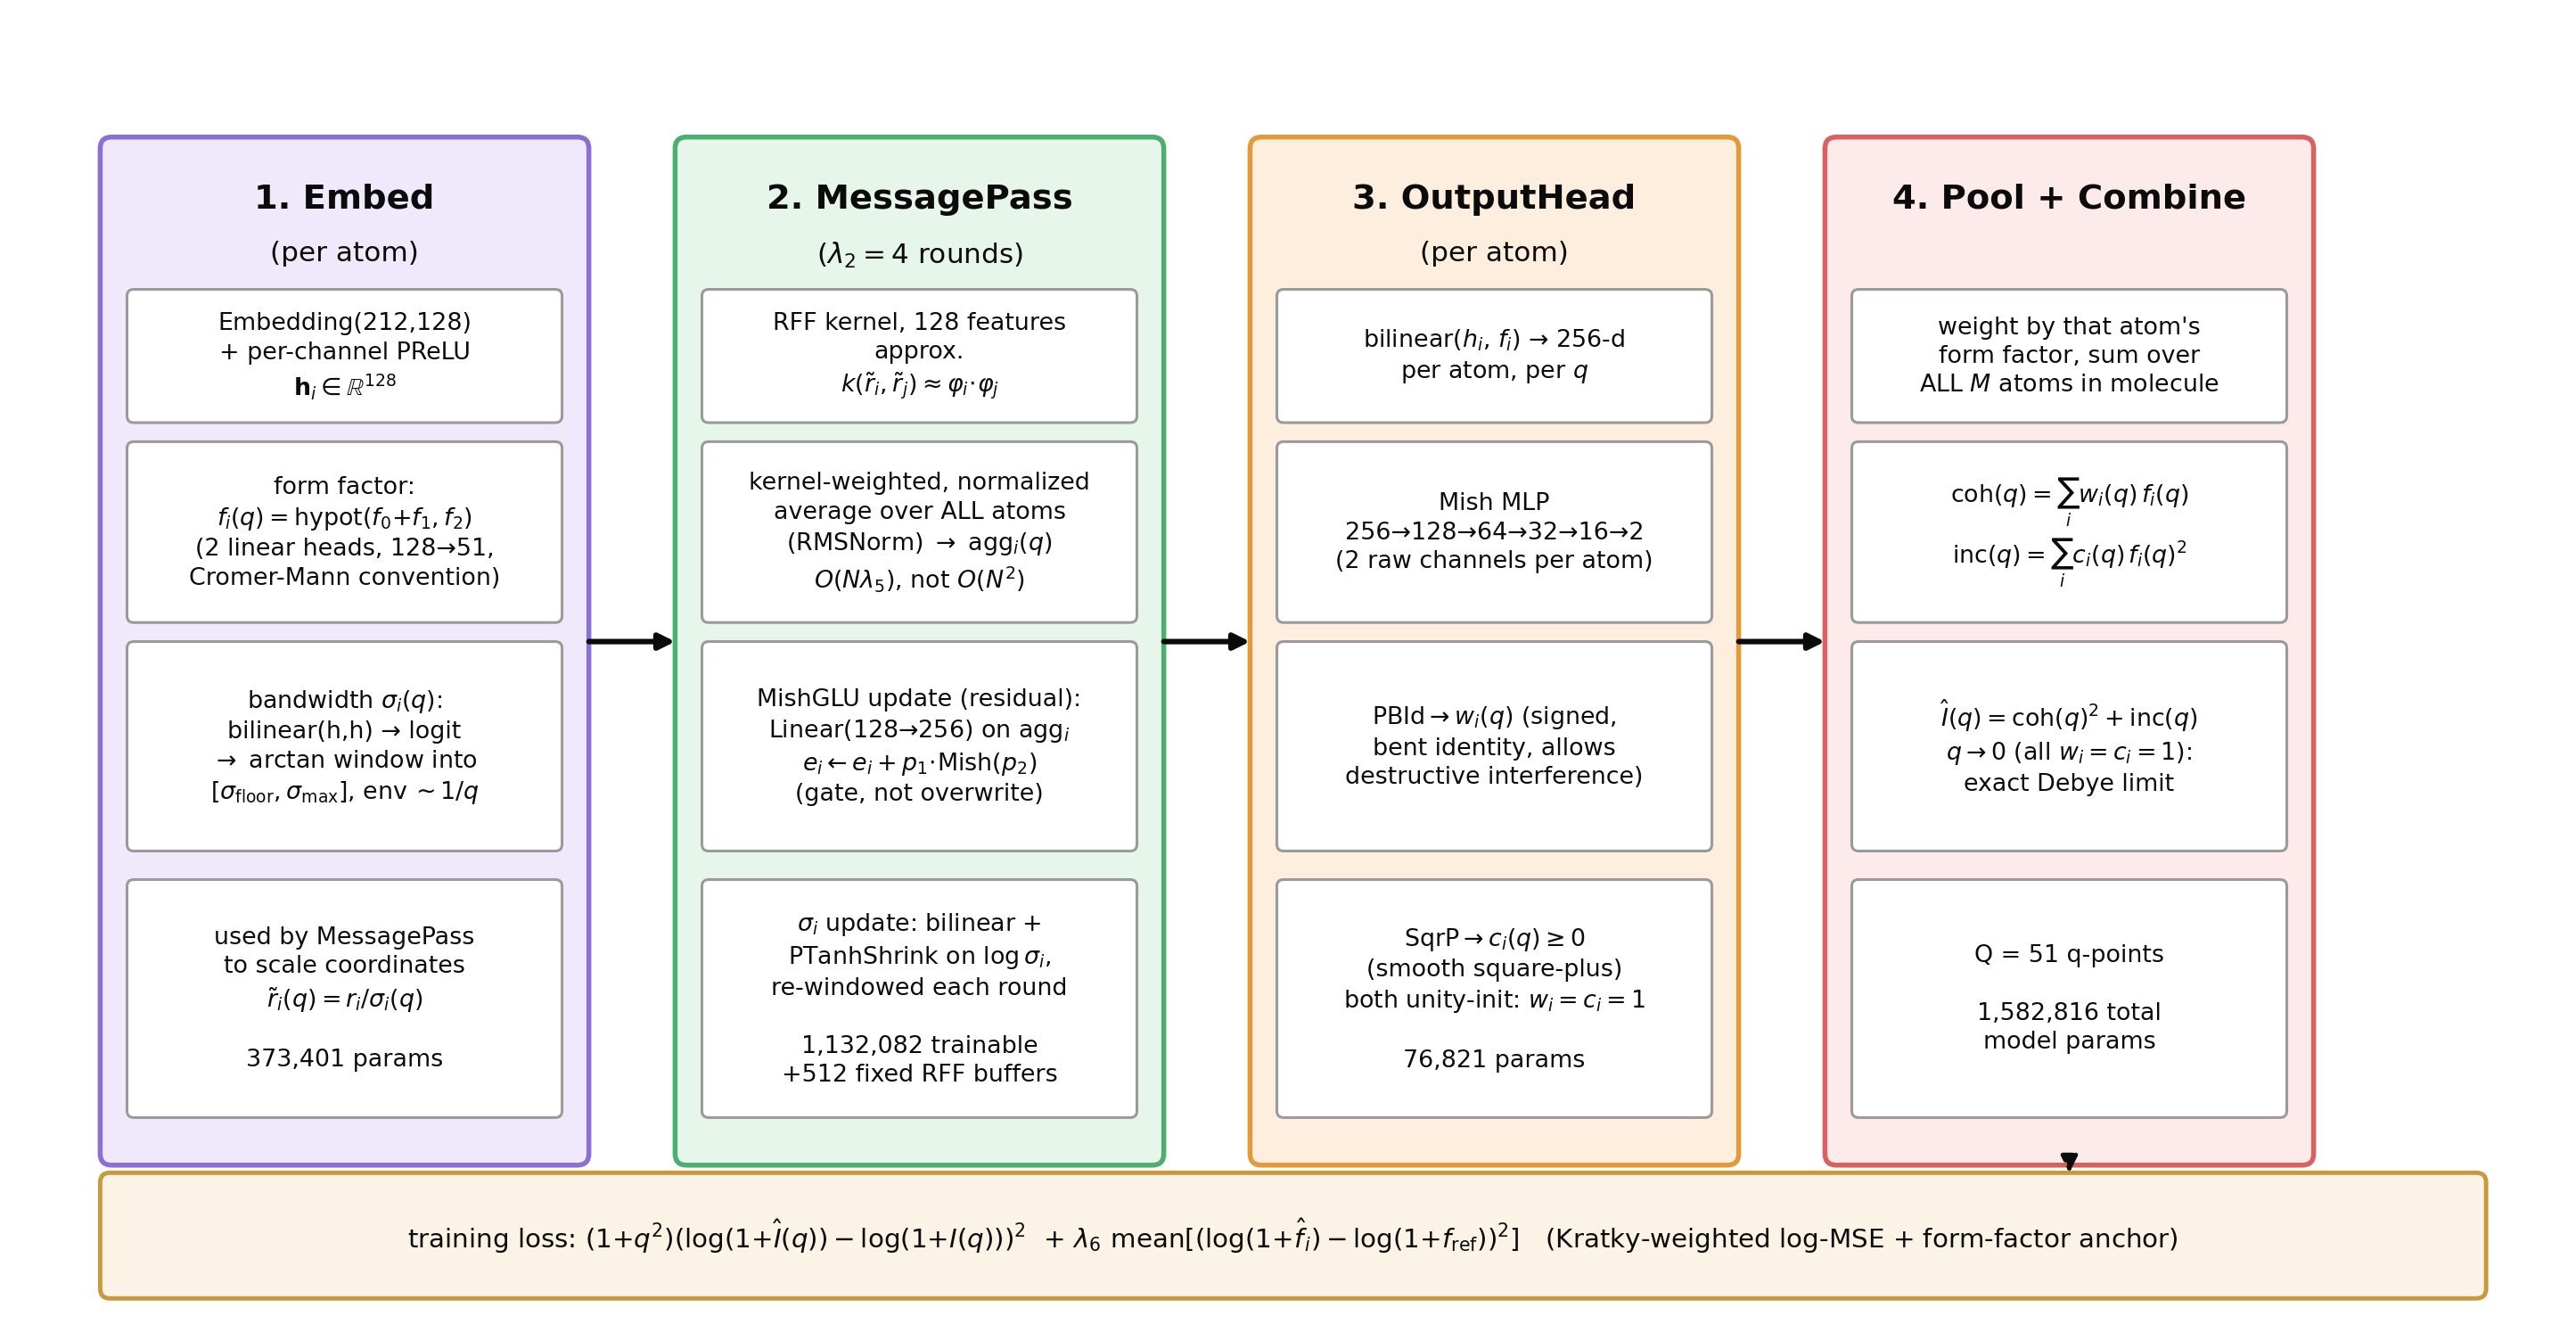
\includegraphics[width=1.25\linewidth ]{figs/architecture.png}
    \caption{Input (atomic coordinates + element types) $\to$ ScatterNet $\to$ output
    $\hat I(q) = \mathrm{coh}(q)^2 + \mathrm{inc}(q)$: per-atom coherent ($w_i$, signed,
    captures destructive interference) and incoherent ($c_i \geq 0$) channels, weighted
    by each atom's form factor and pooled over all atoms in the molecule.}
    \label{fig:arch}
\end{figure}

%==============================================================================
\section{Background \& Related Work}
%==============================================================================
CRYSOL~\cite{svergun_crysol_1995} established the analytic and non-learned spherical-harmonic
decomposition this project uses for ground truth, built on the Stuhrmann
expansion~\cite{Stuhrmann} of the exact Debye sum~\cite{debye}.
Graph neural networks for molecular property prediction were pioneered by
SchNet~\cite{schutt_schnet_2018}. DimeNet~\cite{gasteiger_dimenet_2020}
added bond-angle information, improving accuracy on the QM9 dataset~\cite{ramakrishnan_qm9_2014},
part of which is folded into the training set of ScatterNet. PaiNN~\cite{Schutt2021} extended
message passing to rotationally equivariant properties. None of these five
target $I(q)$ directly as a learned, differentiable quantity; ScatterNet replaces the
$O(N^2)$ analytic sum with an $O(N)$ learned surrogate.

%==============================================================================
\section{Data Processing}
%==============================================================================
A dataset of 1,044,583 molecules spanning 1--6,046 atoms was assembled from 13 sources
(Table~\ref{tab:dataset}), covering 474 unique atom/ion types. 
Raw structures (\texttt{.cif}, \texttt{.pdb}, \texttt{.xyz}) were converted to a 
uniform Cartesian XYZ representation; dummy sites
were removed, deuterium mapped to hydrogen, zero-atom structures discarded, and
non-element placeholders (\texttt{X}, \texttt{M}, \texttt{Cn}) excluded from the
ionic makeup. $I(q)$ for each molecule were calculated, and an `encoding' was calculated,
corresponding to the atom's ionic makeup.

\begin{wraptable}{l}{10cm}
\centering
\small
\caption{Cleaned dataset composition by source.}
\label{tab:dataset}
\begin{tabular}{lrl}
\toprule
Group & Molecules & Atom range \\
\midrule
COD (Crystallography Open Database)     & 532,302 & 1--6,032 \\
QM9 (small organic molecules)           & 133,844 & 3--29 \\
tmQM (transition metal complexes)       & 108,541 & 7--569 \\
rcsb\_sml (PDB, small)                  & 96,158  & 28--6,036 \\
viro3D (viral protein structures)       & 60,488  & 173--6,046 \\
hydration\_shells (water solvation)     & 48,571  & 3--147 \\
rcsb\_med (PDB, medium)                 & 31,749  & 2,996--6,046 \\
mofs (metal-organic frameworks)         & 30,863  & 10--5,760 \\
monoatomic/binary/Si-Ge/Ar-Ne/NaCl clusters & 2,067 & 2--1,482 \\
\midrule
\textbf{Total} & \textbf{1,044,583} & \textbf{1--6,046} \\
\bottomrule
\end{tabular}
\end{wraptable}

$I(q)$ ground truth was computed from the cleaned XYZ via the Stuhrmann decomposition at
$L{=}50$ and stored, together with the coordinates, in a compressed HDF5 database. To
avoid padding waste across a 1--6,046 atom size range, molecules are grouped by size
into 57 atom-count buckets; each bucket is stratified 70/15/15 at the molecule level
into train/val/test independently, so every split contains both small and large
molecules.

%==============================================================================
\section{Architecture}
%==============================================================================
ScatterNet (Fig.~\ref{fig:arch}) has three stages, $Q{=}51$ q-points and a
$212$-entry element vocabulary (211 ions + 1 padding index). \textbf{Embed}
(373,401 params) looks up a learned $\lambda_1{=}128$-d vector per atom
(\texttt{Embedding}$(212,128)$) through a channel-wise \textbf{PReLU}, then splits it
via two linear heads into a complex form-factor magnitude $f_i(q) =
\mathrm{hypot}(f_0{+}f_1,\,f_2)$ and, via a $(128,51,51)$ bilinear layer, 
a kernel-bandwidth logit squashed into  $(\sigma_{\mathrm{floor}},\sigma_{\max})$ 
by a smooth \textbf{arctan} soft window, which was chosen over a hard clamp so gradients 
do not vanish at the boundary. \textbf{MessagePass} ($\lambda_2{=}4$ rounds, 1,132,082 
trainable params $+$ 512 fixed buffers) approximates the Radial Basis Function (RBF)
$k(\tilde r_i,\tilde r_j){\approx}\varphi_i{\cdot}\varphi_j$ between every atom pair via
$\lambda_5{=}128$ fixed Random Fourier Features, cutting the all-pairs cost from
$O(N^2)$ to $O(N\lambda_5)$. Each round, an atom's embedding is updated by a
kernel-weighted, RMSNorm-normalized average over all atoms, fed through a 
\textbf{Mish}-gated GLU ($128{\to}256$, avoids dead units under early, noisy gradients) and added
as a residual, $e_i \leftarrow e_i + \mathrm{gate}_i$. In parallel, a bilinear
layer updates $\log\sigma_i$ each round via \textbf{PTanhShrink} ($f(y){=}y-c\tanh(y/c)$,
learned width $c$, shrinks small noisy updates toward zero), re-windowed by the same
arctan squash as Embed. \textbf{OutputHead} (76,821 params) bilinearly combines each
atom's updated embedding with its own $f_i(q)$, narrows through a Mish MLP
($256{\to}128{\to}64{\to}32{\to}16{\to}2$) to two channels, then
\textbf{PBId} gives $w_i(q)$ and \textbf{SqrP} (square-plus, strictly $\geq 0$) 
gives $c_i(q)$; both  unity-initialized ($w_i{=}c_i{=}1$). 
Only in the final \textbf{pooling} step are atoms
combined: each channel is weighted by that atom's own form factor and summed over all
$M$ atoms, $\mathrm{coh}(q){=}\sum_i w_i(q)f_i(q)$, $\mathrm{inc}(q){=}\sum_i
c_i(q)f_i(q)^2$, giving $\hat I(q) = \mathrm{coh}(q)^2 + \mathrm{inc}(q)$. \textbf{Total: 1,582,816
parameters} (1,582,304 trainable $+$ 512 fixed).

Training minimizes a Kratky-weighted log-MSE, $(1+q^2)(\log(1{+}\hat I(q)) -
\log(1{+}I(q)))^2$, plus a form-factor penalty ($\lambda_6{=}1.0$, anchoring
$\hat f_i(q)$ to tabulated \texttt{xraydb} values), via AdamW
($\mathrm{lr}=1.3\times10^{-4}$, weight decay $0.1$, ReduceLROnPlateau, grad clip $1.0$),
tensor/data-parallel routed across 2$\times$T4 GPUs by bucket atom-count
($\mathtt{dp\_atom\_threshold}{=}101$).

%==============================================================================
\section{Baseline Model}
%==============================================================================
Nine non-GNN baselines were implemented: closed-form physics fits per-molecule
(Guinier, Guinier-Porod, a binned Debye sum over the histogrammed pairwise-distance
distribution $P(r)$, recovering the exact Debye equation as bin count grows),
stochastic estimators subsampling the $O(N^2)$ pairwise sum (\texttt{propoEst},
\texttt{stratEst}), and learned baselines with no 3-D access (a training-mean-by-
atom-count lookup, a linear SVM over composition, a 2-layer MLP over composition +
size). Beating Binned Debye (closest coarse-graining of the ground truth, thus a
feasibility ceiling) is not the bar; beating the composition-only baselines is, since
that proves genuine 3-D structure use rather than size or composition alone.

%==============================================================================
\section{Quantitative Results}
%==============================================================================
Training reached epoch 33 (Fig.~\ref{fig:loss}); test-set MSLE $= 0.115$ at
71.1~$\mu$s/atom inference (Table~\ref{tab:quant}). This already beats every
composition-only baseline (Atom-Count, Linear SVM, MLP, Nearest-Neighbour) and the
Guinier physics fits, confirming the model learning genuine 3-D structure. It
still trails Binned Debye and \texttt{stratEst}, the two baselines with explicit
pairwise-distance access. Only 5\% of the dataset is drawn per epoch. An epoch trained
on 100\% of the dataset took around 12 hours to complete on the available 2$\times$T4 GPUs.
This may explain the visible plateaus and short 
reversals in Fig.~\ref{fig:loss} (e.g.\ epochs 10--11, 14, 18).

\begin{table}[h]
\centering
\begin{minipage}{0.42\linewidth}
    \centering\small
    \captionof{table}{ScatterNet (epoch 33) vs.\ baseline anchors, by MSLE.}
    \label{tab:quant}
    \begin{tabular}{lr}
    \toprule
    Model & MSLE \\
    \midrule
    Binned Debye (ceiling)      & 0.0053 \\
    SAXS \texttt{stratEst}      & 0.0531 \\
    \textbf{ScatterNet (epoch 33)} & \textbf{0.115} \\
    Guinier-Porod               & 0.346 \\
    SAXS \texttt{propoEst}      & 0.366 \\
    Linear SVM                  & 0.772 \\
    Atom-Count                  & 1.010 \\
    MLP                         & 1.821 \\
    \bottomrule
    \end{tabular}
\end{minipage}\hfill
\begin{minipage}{0.54\linewidth}
    \centering
    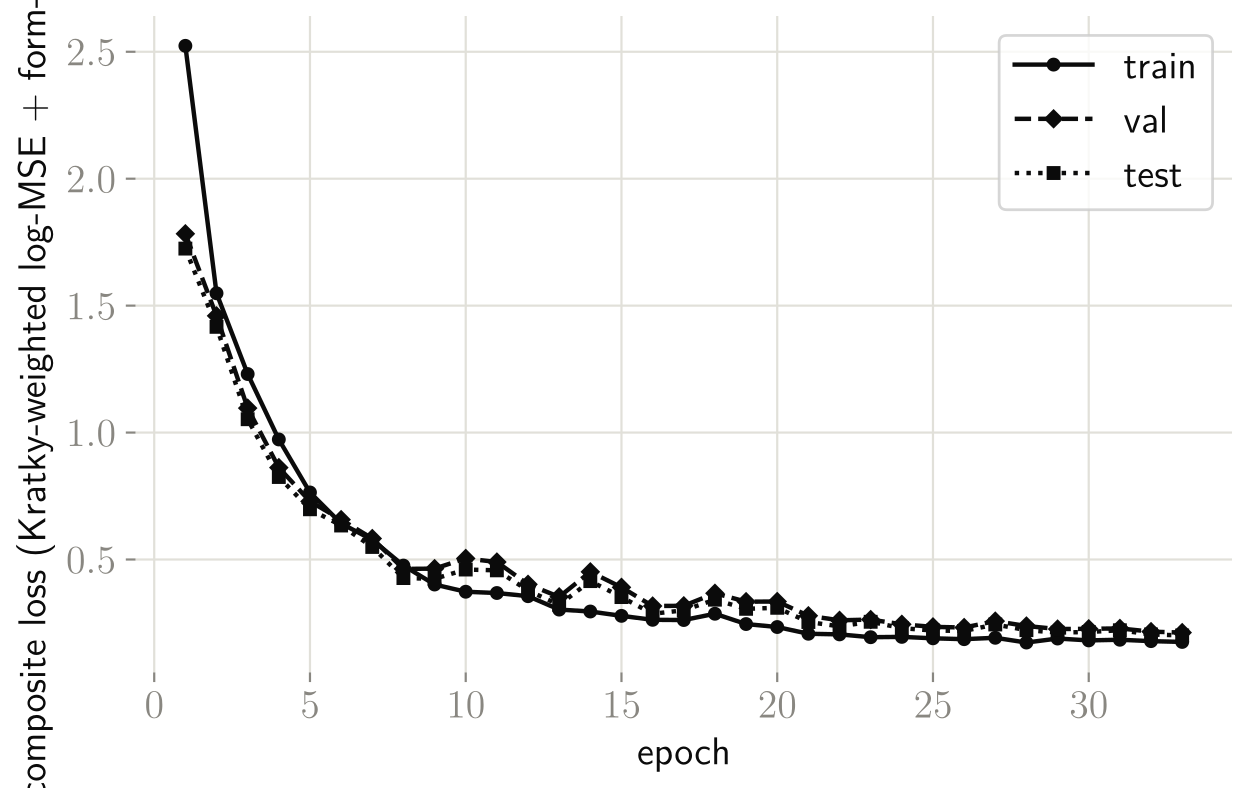
\includegraphics[width=\linewidth]{figs/loss_per_epoch_full.png}
    \vspace{2mm} 
    \captionof{figure}{Composite train/val/test loss across 33 epochs.}
    \label{fig:loss}
\end{minipage}
\end{table}

\begin{figure}[h]
    \centering
    \begin{minipage}{0.48\linewidth}
        \centering
        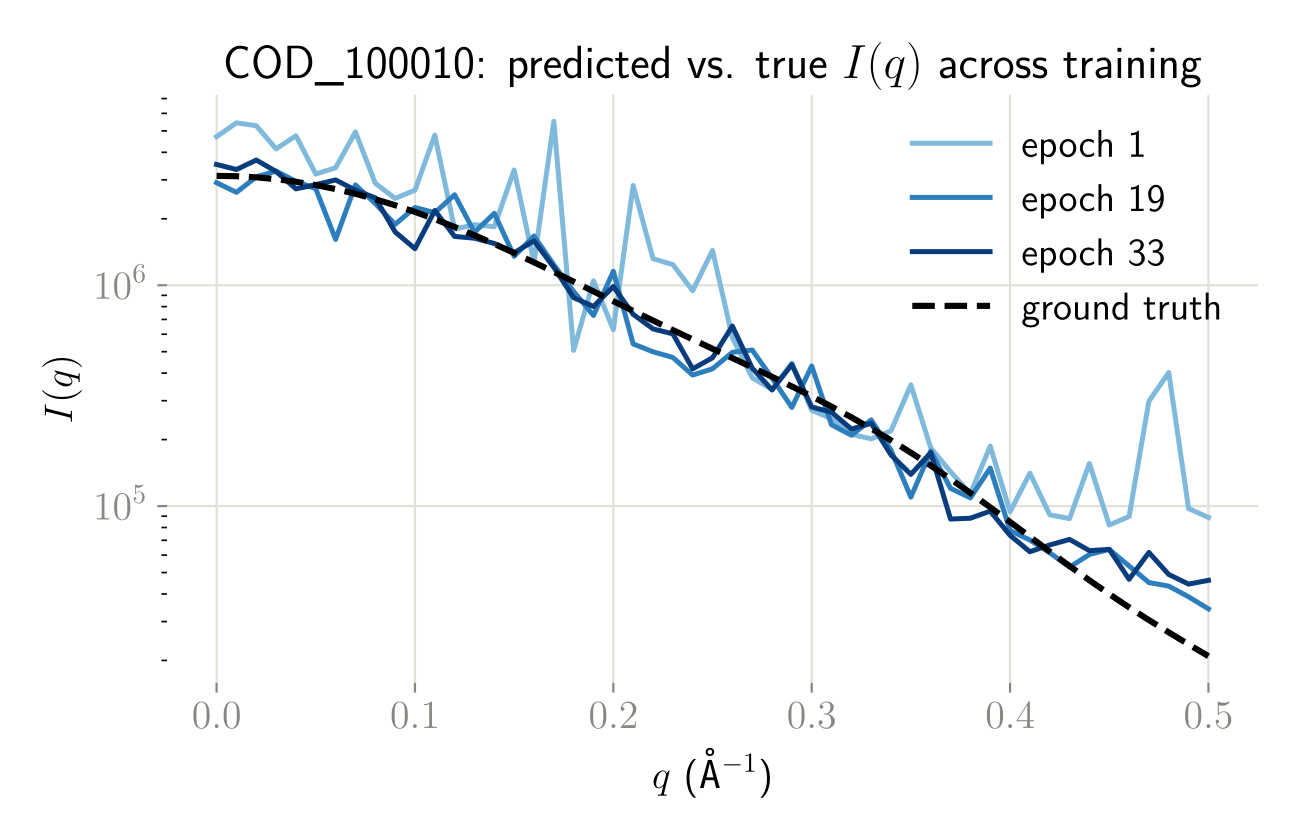
\includegraphics[width=\linewidth]{figs/predicted_vs_true_epochs.png}
        \\[1pt]{\small (a) predicted vs.\ true $I(q)$}
    \end{minipage}\hfill
    \begin{minipage}{0.48\linewidth}
        \centering
        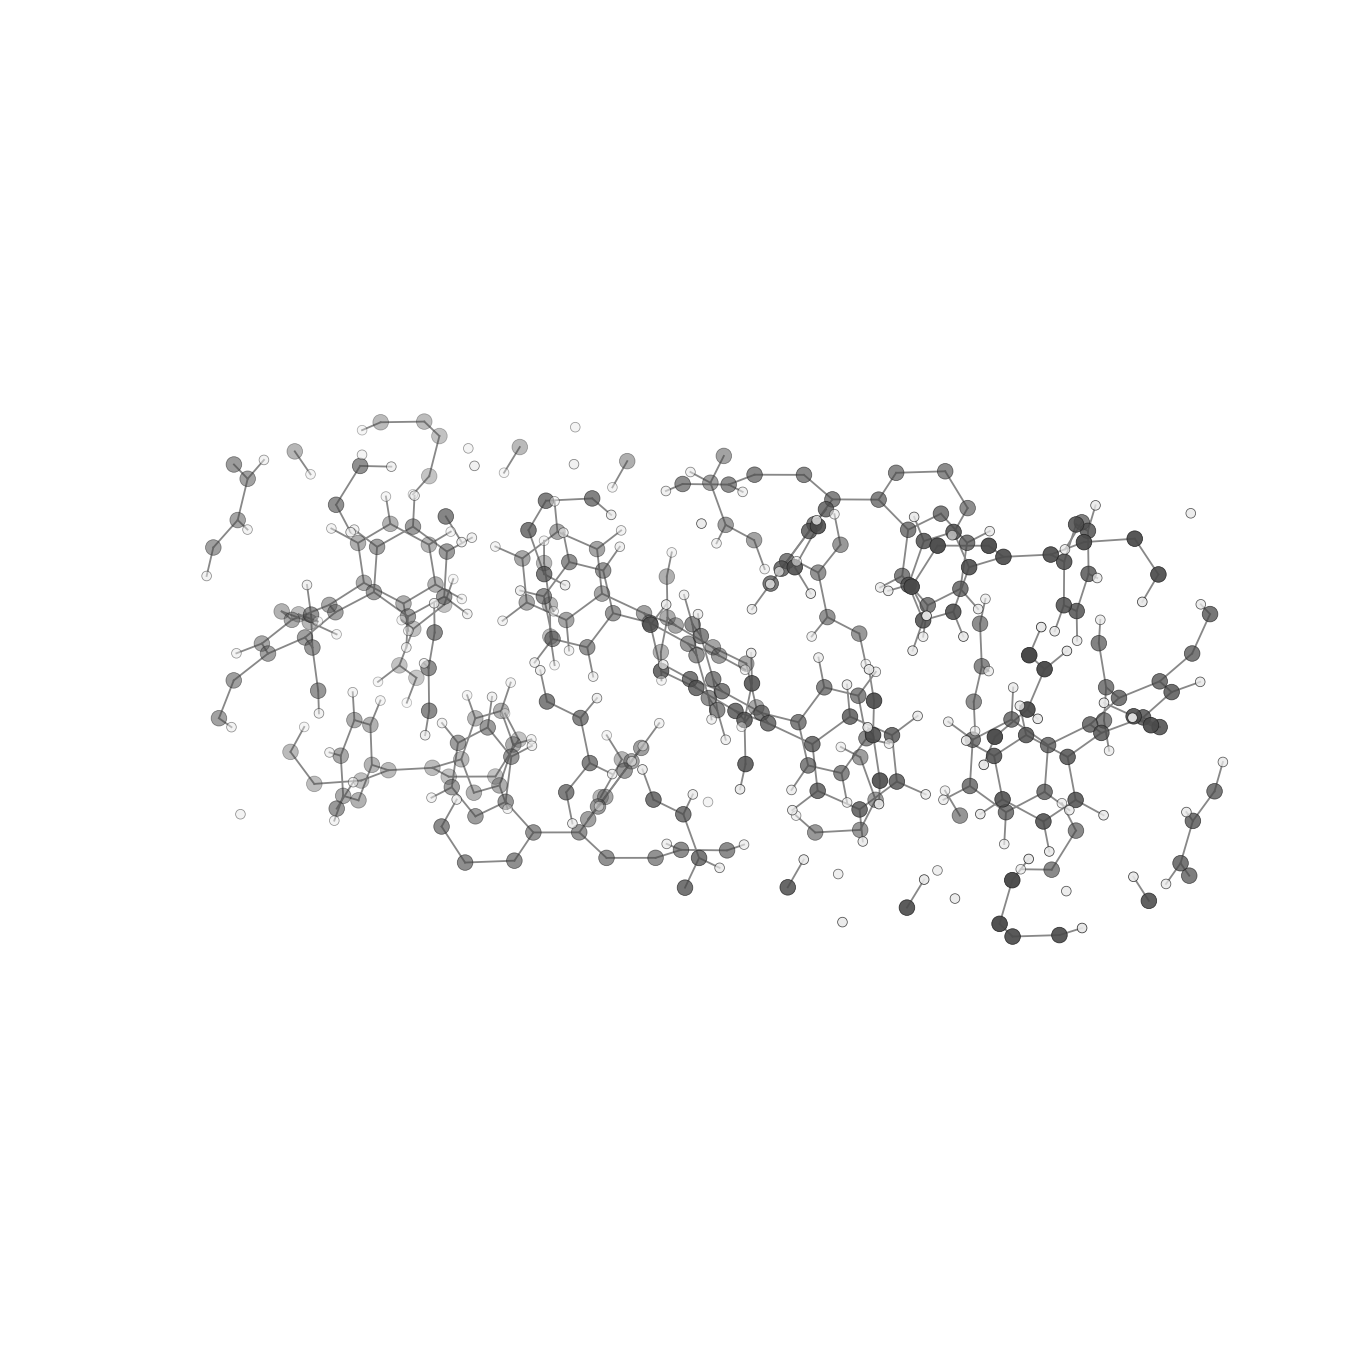
\includegraphics[width=\linewidth]{figs/cod_100010_structure.png}
        \\[1pt]{\small (b) COD\_100010 (448 atoms)}
    \end{minipage}
    \caption{(a) Predicted vs.\ true $I(q)$ for the crystal structure in (b), epochs
    1/19/33; whole-curve mean log-space error falls monotonically,
    $0.55\to0.20\to0.19$ (relative error $117\%\to21.5\%\to21.3\%$), tracking ground
    truth closely by epoch 19; only $q{=}0$ itself is non-monotonic
    ($50\%\to7\%\to13\%$), consistent with Fig.~\ref{fig:loss}'s per-epoch sampling
    noise. (b) A unit cell (C\textsubscript{264}H\textsubscript{184}), several distinct aromatic
    organic molecules.}
    \label{fig:predtrue}
\end{figure}

\vspace{-15pt}
%==============================================================================
\section{Qualitative Results}
%==============================================================================
Fig.~\ref{fig:predtrue}(b) shows predicted-vs-true $I(q)$ convergence over training on
a held-out crystal structure. Per-$q$ error across the full test set follows the same
pattern (Fig.~\ref{fig:qual}).
\begin{wrapfigure}{l}{0.75\linewidth}
    \centering
    \begin{minipage}{0.75\linewidth}
        \centering
        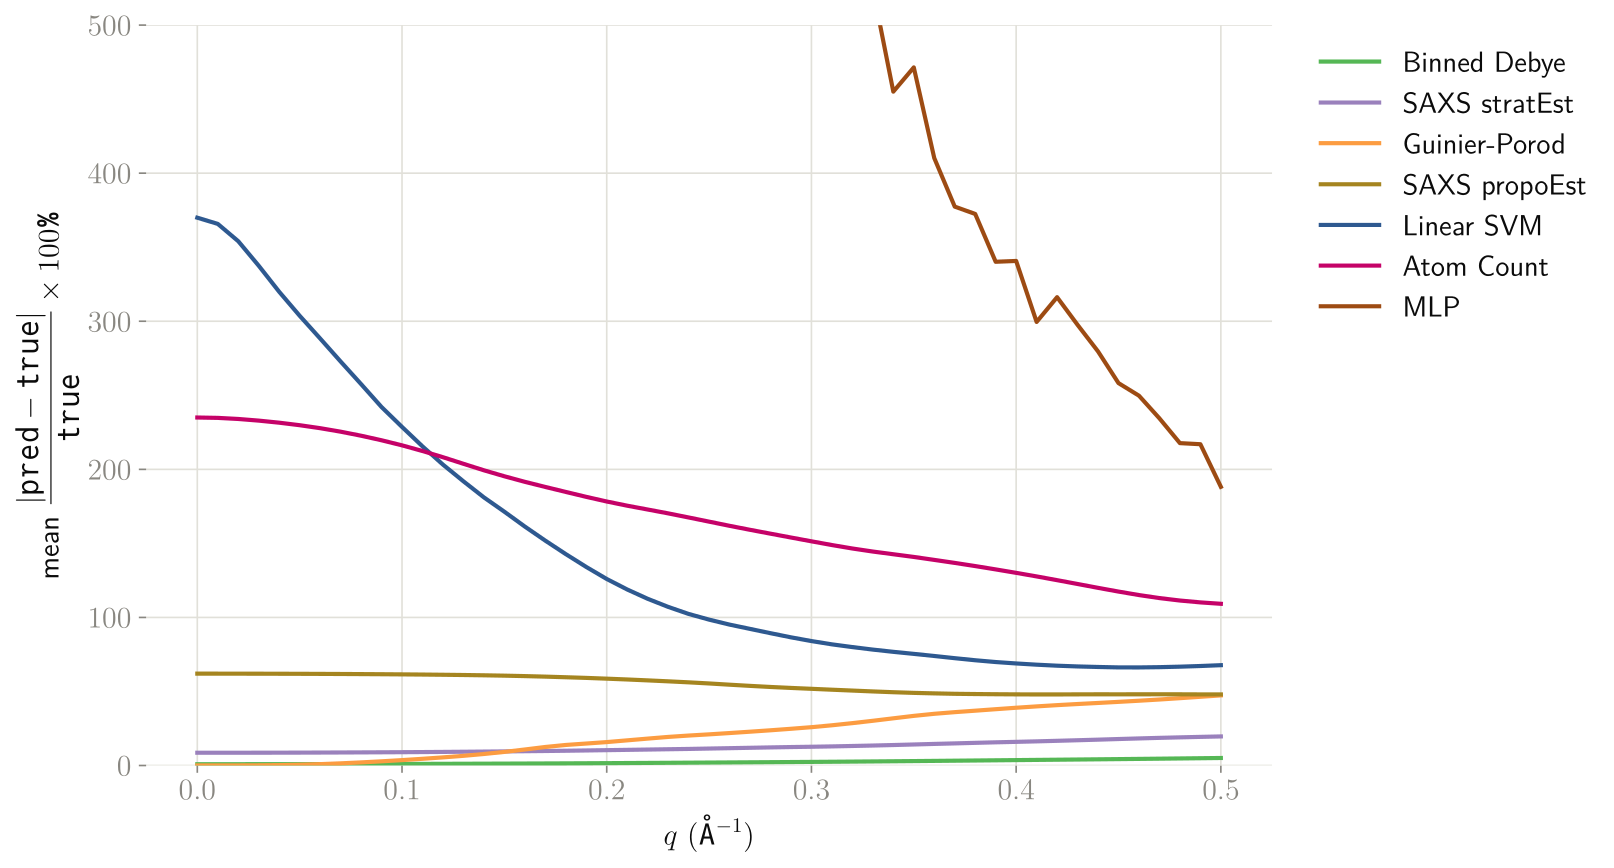
\includegraphics[width=\linewidth]{figs/baseline_per_q_percent_error.png}
        \\[1pt]{\small (a) baselines}
    \end{minipage}\hfill
    \begin{minipage}{0.75\linewidth}
        \centering
        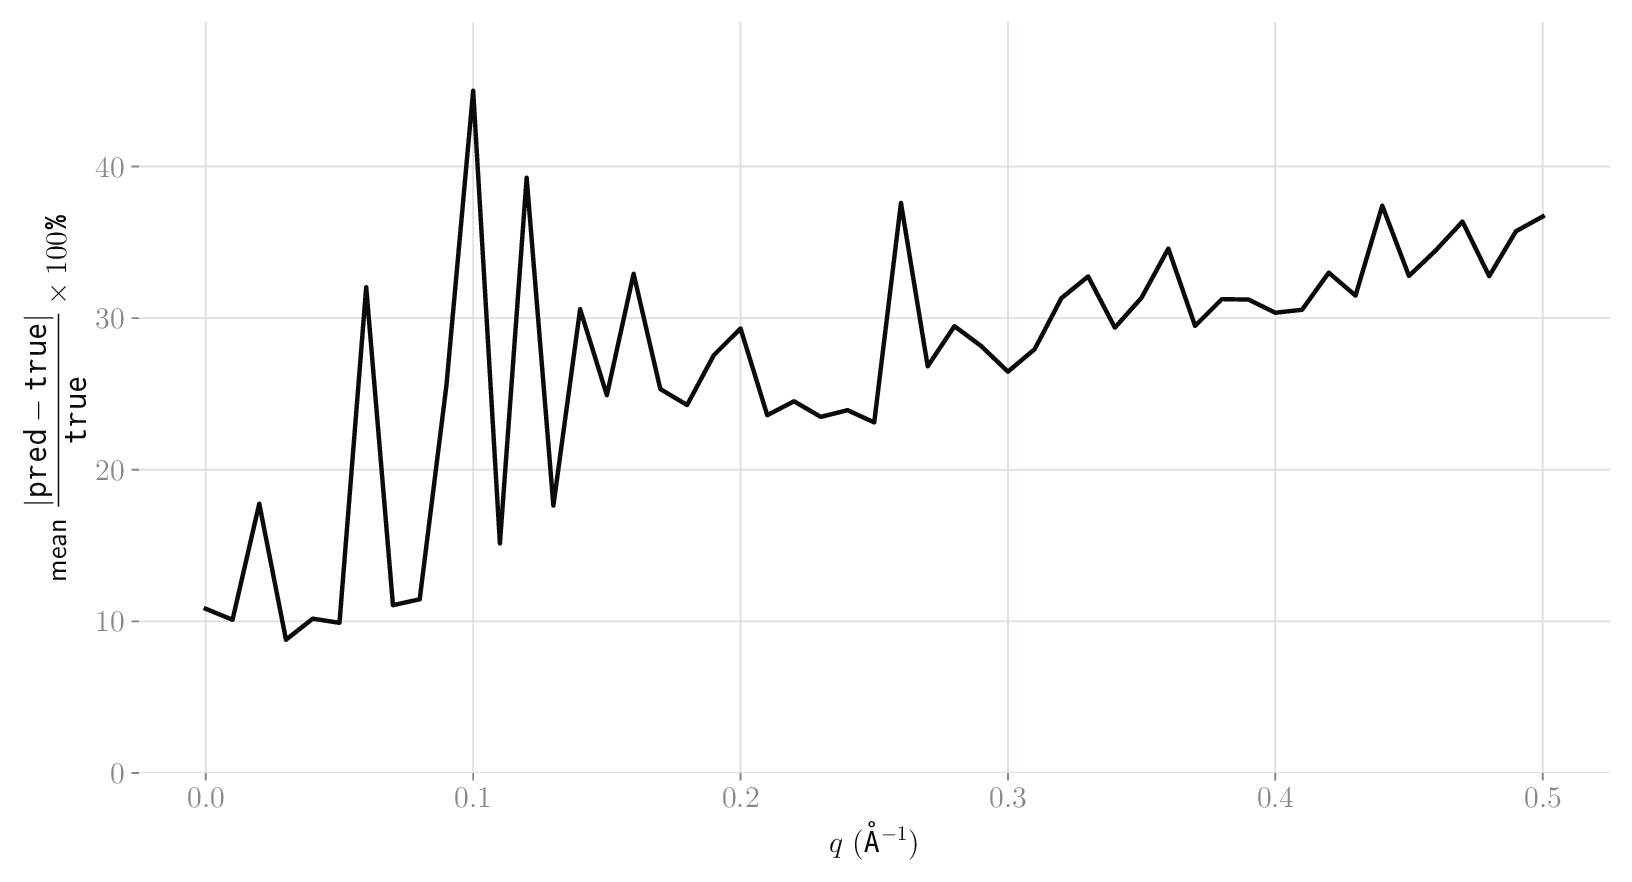
\includegraphics[width=\linewidth]{figs/scatternet_per_q_percent_error.png}
        \\[1pt]{\small (b) ScatterNet}
    \end{minipage}
    \caption{Per-$q$ mean \% error: baselines (a) vs.\ ScatterNet (b, epoch 33). Mean
    per-$q$ $R^2{=}0.965$ (worst $0.917$); mean error $27.0\%$, rising to $32.9\%$ at
    high $q$.}
    \label{fig:qual}
\end{wrapfigure}

%==============================================================================
\section{Evaluate Model on New Data}
%==============================================================================
See: Fig.~\ref{fig:predtrue}'s structure ran through inference code independent of the
training/val/test split.

%==============================================================================
\section{Discussion}
\label{sec:discussion}
%==============================================================================
ScatterNet already beats every baseline that don't compute pairwise distances,
despite the baselines using 10\% of the dataset whereas ScatterNet trained on 5\%.
It still trails Binned Debye and \texttt{stratEst}
(Table~\ref{tab:quant}); the gap concentrates in the low-$q$/Guinier-region magnitude (Fig.~\ref{fig:predtrue})
and high-$q$ fine structure (Fig.~\ref{fig:qual}), not uniformly across the curve.

(\textbf{channel drift}): the coherent PBId bend weight relaxed $0.98\to0.74$ 
(more linear, less bent);
the incoherent SqrP width shrank $4.0\to2.23$ (sharper positivity floor); and the
largest relative movement was in MessagePass's later-round sigma-bilinear layers.

%==============================================================================
\section{Ethical Considerations}
%==============================================================================
All training data is open-source and fully attributed; no private/sensitive
information is involved.

%==============================================================================
\section{Project Difficulty / Quality}
%==============================================================================
Three factors  made this very difficult. First, The $O(N)$
ground-truth pipeline (Stuhrmann, not naive Debye) and a two-channel head whose
$q{\to}0$ limit is derivedticallyanaly from the Debye equation
(Fig.~\ref{fig:arch}) required deriving the underlying physic, from first principles. 
Aditionally, the math behind the RFF approximation and the resulting einsums which were 
needed to accumulate the sums were difficult to learn. Second, on 2$\times$T4's 16GB/GPU 
ceiling, real runs OOM'd and ran extremley slow
repeatedly from activation memory  before any model issue were made. 
Fixing it took engineering chunking across multiple axes, tensor/data parallelism,
implementing torch compile, and implementing a custum billinear layer which avoids 
CUDA kernel launches. Third, even at 5\% coverage, epochs take $\sim$1hr
so every hyperparameter changes h ad to be deliberate and the majority of runs had
to be terminated before completion.
(Table~\ref{tab:quant}).

\newpage
\bibliographystyle{unsrtnat}
\bibliography{ref}
\end{document}
